%!Tex Root = ../main.tex
% ./Packete.tex
% ./Design.tex
% ./Vorbereitung.tex
% ./Aufgabe1.tex
% ./Aufgabe2.tex
% ./Aufgabe3.tex
% ./Aufgabe4.tex
% ./Appendix.tex

\begin{mindmap}
  \begin{mindmapcontent}
    \node (be) at (current page.center) {Beweisen}
    child {
      node {Induktion}
      child {
        node {Vollständige Induktion
          \resizebox{\textwidth}{!}{
            \begin{minipage}[t]{16cm}
              \begin{itemize}
                \item für \alert{Allbehauptungen}: $\forall n\in\mathbb{N}:\mathcal{E}(n)$ (Eigenschaft $\mathcal{E}$)
                \item die allgemeine Form wird als \alert{Strukturelle Induktion} bezeichnet, \alert{Vollständige Induktion} ist zum Beweis von Aussagen für alle Natürlichen Zahlen
                \begin{itemize}
                  \item Menge der \alert{natürlichen Zahlen} $\mathbb{N}$ weißt geignete Struktur auf, da auf ihnen die Nachfolgerbeziehung besteht
                \end{itemize}
                \item man führt Teilbewise für $2$ Fälle: 
                \begin{itemize}
                  \item \alert{Basisfall:} ${\mathcal{E}}(0)$, d.h. die natürliche Zahl $0$ hat die Eigenschaft $\epsilon$
                  \item \alert{Induktionsfall:} $\forall i\in\mathbb{N} \left(\mathcal{E}(i)\Rightarrow\mathcal{E}(i+1)\right)$, d.h. die Eigenschaft $\epsilon$ überträgt sich von jeder natürlichen Zahl $i$ auf ihren Nachfolger $i + 1$
                \end{itemize}
                \item bei beweisender Allbehauptung für den Induktionsfall wird Implikation: Sei $i\in\mathbb{N}$ beliebig. Zu zeigen: $\epsilon(i)\Rightarrow\epsilon(i+1)$ zerlegt in: Sei $i\in\mathbb{N}$ beliebig. Es gelte: $\epsilon(i)$. Zu zeigen: $\epsilon(i+1)$
                \item Diese Darstellung des Induktionsfalls legt seine Zerlegung in die üblichen drei Bestandteile \alert{Induktionsannahme}, \alert{Induktionsbehauptung}, \alert{Induktionsschritt} nahe:
              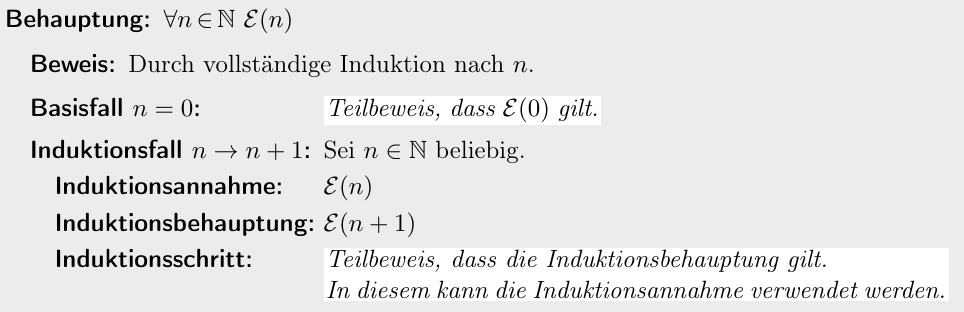
\includegraphics[width=\linewidth]{./figures/vollstaendige_induktion.png}
              \end{itemize}
              \begin{itemize}
                \item Induktionsfall beweist Allbehauptung mit darin enthaltener Implikationsbehauptung 
                \item Wenn für Eigenschaft $\epsilon$ Basisfall und Induktionsfall bewiesen sind, gilt, dass jede natürliche Zahl die Eigenschaft $\epsilon$ hat, denn:
                \begin{enumerate}
                  \setcounter{enumi}{-1}
                  \item Wegen des Basisfalls gilt $\epsilon(0)$.
                  \item Mit $\epsilon(0)$ gilt wegen des Induktionsfalls auch $\epsilon(1)$.
                  \item Mit $\epsilon(1)$ gilt wegen des Induktionsfalls auch $\epsilon(2)$.
                  \item Mit $\epsilon(2)$ gilt wegen des Induktionsfalls auch $\epsilon(3)$.
                  \item $\ldots$
                \end{enumerate}
              \end{itemize}
              \includegraphics[width=0.6\textwidth]{./figures/vollständige_induktion_1.png}\\
              \includegraphics[width=0.8\textwidth]{./figures/vollständige_induktion_2.png}
            \end{minipage}
          }
        }
      }
    }
    child {
      node {Indirekter Beweis}
      child {
        node {Beweis durch Widerspruch
          \resizebox{\textwidth}{!}{
            \begin{minipage}[t]{16cm}
              \begin{itemize}
                \item anstatt einen mathematischen Satz $S$ direkt zu beweisen, kann man seine Negation $\neg S$ durch logische Schlussfolgerungen zu einem Widerspruch führen.
                \item Wenn man die Widerspruchsanahme $\neg S$ zu einem Widerspruch geführt hat, weiß man, dass $\neg S$ immer falsch sein muss. Damit ist die doppelte Negation $\neg\neg S$ von $S$ wahr. Da $\neg\neg S \Leftrightarrow S$ eine Tautologie ist, ist $\neg\neg S$ genau dann wahr, wenn $S$ wahr ist. Damit muss $S$ wahr sein.
                \item \alert{Zerlegung der Implikation:}
                \begin{align*}
                  &V o r a u s s e t z u n g_{1}\wedge\cdot\cdot\cdot\wedge\;V o r a u s s e t z u n g_{n}\rightarrow B e h a u p t u n g\\
                  &\Leftrightarrow \neg\left(V o r a u s s e t z u n g_{1}\wedge\cdot\cdot\cdot\wedge\ V o r a u s s e t z u n g_{n}\right)\vee B e h a u p t u n g\\
                  &\Leftrightarrow \neg\left(\left(V o r a u s s e t z u n g_{1}\wedge\cdot\cdot\cdot\wedge\;V o r a u s s e t z u n g_{n}\right)\wedge\neg B e h a u p t u n g\right)\\
                  &\Leftrightarrow V o r a u s s e t z u n g_{1}\wedge\cdot\cdot\cdot\wedge\ V o r a u s s e t z u n g_{n}\wedge\lnot B e h a u p t u n g \rightarrow \perp
                \end{align*}
                \begin{itemize}
                  \item \alert{Anders gesagt:} Aus den Vorraussetzungen folgt logisch die Behauptung \textit{genau dann wenn} $V o r a u s s e t z u n g_{1}\wedge\cdot\cdot\cdot\wedge\ V o r a u s s e t z u n g_{n}\wedge\lnot B e h a u p t u n g$ \textit{NICHT} gilt.
                \end{itemize}
              \end{itemize}
              \begin{itemize}
                \item es gibt neben \alert{expliziten Voraussetzungen} auch \alert{implizite Voraussetzungen}, die nicht ausdrücklich genannt werden (Rechenregeln und Standard-Definitionen)
                \item In der \alert{Behauptung} steht immer eine \alert{wahre Aussage}. Hat man eine Aussage, die \alert{nicht wahr} ist, muss man sie \alert{negiert} in die Behauptung schreiben.
              \end{itemize}
              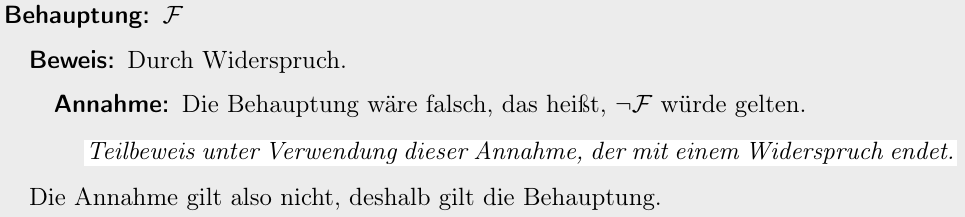
\includegraphics[width=\textwidth, center]{./figures/beweis_durch_widerspruch.png}\\
              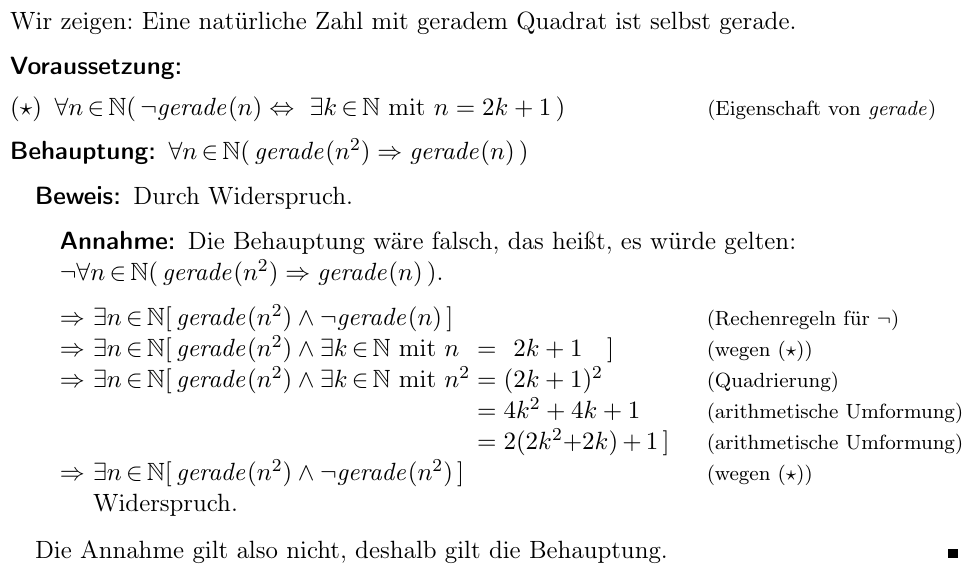
\includegraphics[width=0.7\textwidth, center]{./figures/beweis_durch_widerspruch_beispiel.png}
            \end{minipage}
          }
        }
      }
      child {
        node {Beweis durch Kontraposition
          \resizebox{\textwidth}{!}{
            \begin{minipage}[t]{8cm}
              \begin{itemize}
                \item $\mathcal{F}\rightarrow\mathcal{G}\Leftrightarrow\neg\mathcal{F}\vee\mathcal{G}\Leftrightarrow\neg\neg\mathcal{G}\vee¬\mathcal{F}\Leftrightarrow\neg\mathcal{G}\rightarrow\neg\mathcal{F}$
                \item Konstraposition der Behauptung, die eine Implikation ist wird bewiesen. Immer mit Beweismuster für Implikation kombiniert, da Kontraposition der Behauptung auch eine Implikation ist
              \end{itemize}
              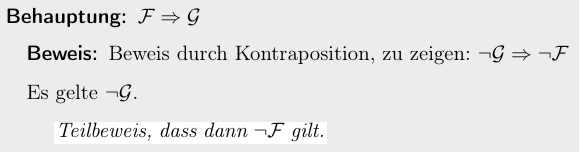
\includegraphics[width=0.6\textwidth, center]{./figures/kontraposition.png}\\
              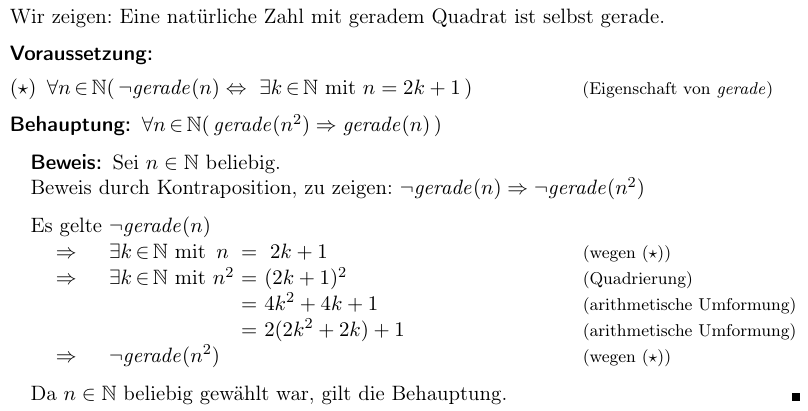
\includegraphics[width=0.8\textwidth, center]{./figures/kontraposition_example.png}
            \end{minipage}
          }
        }
      }
    };
  \end{mindmapcontent}
  % \begin{edges}
  %   \edge{test}{re}
  % \end{edges}
  \annotation{be.south}{This mindmap is provided without guarantee of correctness and completeness!}
  \annotation{be.north}{\href{/tmp/current.pdf}{go back}}
\end{mindmap}
